%Este trabalho está licenciado sob a Licença Atribuição-CompartilhaIgual 4.0 Internacional Creative Commons. Para visualizar uma cópia desta licença, visite http://creativecommons.org/licenses/by-sa/4.0/deed.pt_BR ou mande uma carta para Creative Commons, PO Box 1866, Mountain View, CA 94042, USA.

\chapter{Equações Diferenciais Parciais}\label{cap_edp}
\thispagestyle{fancy}

Neste capítulo, discutimos alguns tópicos fundamentais da aplicação do método de diferenças finitas para a simulação (aproximação da solução) de equações diferenciais parciais.

\section{Equação de Poisson}\label{cap_edp_sec_Poisson}\index{equação! de Poisson}

A equação de Poisson em um domínio retangular $D = (x_{\text{ini}}, x_{\text{fin}})\times (y_{\text{ini}}, y_{\text{fin}})$ com condições de contorno de Dirichlet homogêneas refere-se o seguinte problema
\begin{align}
  u_{xx} + u_{yy} &= f(x, y),~(x, y)\in D, \label{eq:edp_Poisson_eq}\\
  u(x_{\text{ini}}, y) &= 0,~y_{\text{ini}}\leq y \leq y_{\text{fin}},\label{eq:edp_Poisson_bcxini}\\
  u(x_{\text{fin}}, y) &= 0,~y_{\text{ini}}\leq y \leq y_{\text{fin}},\label{eq:edp_Poisson_bcxfin}\\
  u(x, y_{\text{ini}}) &= 0,~x_{\text{ini}}\leq x \leq x_{\text{fin}},\label{eq:edp_Poisson_bcyini}\\
  u(x, y_{\text{fin}}) &= 0,,~x_{\text{ini}}\leq x \leq x_{\text{fin}},\label{eq:edp_Poisson_bcyfin}
\end{align}
onde $u = u(x,y)$ é a incógnita.

A aplicação do método de diferenças finitas para resolver este problema consiste dos mesmos passos usados para resolver problemas de valores de contorno (veja Capítulo~\ref{cap_pvc}), a saber: 1. construção da malha, 2. discretização das equações, 3. resolução do problema discreto.

\begin{flushleft}
  {\bf 1. Construção da malha}
\end{flushleft}

Tratando-se do domínio retangular $\overline{D} = [x_{\text{ini}}, x_{\text{fin}}]\times [y_{\text{ini}}, y_{\text{fin}}]$, podemos construir uma malha do produto cartesiano de partições uniformes dos intervalos $[x_{\text{ini}}, x_{\text{fin}}]$ e $[y_{\text{ini}}, y_{\text{fin}}]$. Mais explicitamente, tomamos
\begin{align}
  x_{i} &:= x_{\text{ini}} + (i-1)h_x,\quad h_x = \frac{x_{\text{fin}}-x_{\text{ini}}}{n_x-1},\\
  y_{j} &:= y_{\text{ini}} + (j-1)h_y,\quad h_y = \frac{y_{\text{fin}}-y_{\text{ini}}}{n_y-1},  
\end{align}
onde $i = 1, 2, \dotsc, n_x$, $j = 1, 2, \dotsc, n_y$, sendo $n_x$ e $n_y$ o número de subintervalos escolhidos para as partições em $x$ e $y$, respectivamente.

O produto cartesiano das partições em $x$ e $y$ nos fornece uma partição do domínio $\overline{D}$ da forma
\begin{equation}
  P(\overline{D}) = \{(x_1, y_1), (x_1, y_2), \dotsc, (x_i, y_j), \dotsc, (x_{n_x}, y_{n_y})\},
\end{equation}
cujos nodos $(x_i, y_j)$ podem ser indexados (enumerados) por $k = j + (i-1)n_x$.  Por simplicidade, no decorrer do texto, assumiremos $n_x=n_y=:n$ e, por conseguinte, $h_x=h_y=h$.

\begin{flushleft}
  {\bf 2. Discretização das equações}
\end{flushleft}

Usando a fórmula de diferenças finitas central de ordem $h^2$ para a segunda derivada, temos
\begin{align}
  u_{xx}(x,y) &= \frac{u(x+h,y)-2u(x,y)+u(x-h,y)}{h^2} + O(h^2),\\
  u_{yy}(x,y) &= \frac{u(x,y+h)-2u(x,y)+u(x,y-h)}{h^2} + O(h^2).
\end{align}
Daí, denotando $u_{ij}\approx u(x_i, y_j)$ temos
\begin{align}
  u_{xx}(x_i,y_j) &= \frac{u_{i+1,j}-2u_{i,j}+u_{i-1,j}}{h^2} + O(h^2),\\
  u_{yy}(x_i,y_j) &= \frac{u_{i,j+1}-2u_{i,j}+u_{i,j-1}}{h^2} + O(h^2).  
\end{align}
Então, da equação~\ref{eq:edp_Poisson_eq} temos
\begin{equation}
  \frac{u_{i+1,j}-2u_{i,j}+u_{i-1,j}}{h^2} + \frac{u_{i,j+1}-2u_{i,j}+u_{i,j-1}}{h^2} + O(h^2) = f(x_i,y_j).
\end{equation}
Adora, denotando $u_k := u_{j+(i-1)n}$, desprezando o termo do erro de truncamento e rearranjando os termos nesta última equação temos
\begin{equation}\label{eq:edp_Poisson_mdf_sis0}
  \frac{1}{h^2}u_{k-n} + \frac{1}{h^2}u_{k-1} -\frac{4}{h^2}u_{k} + \frac{1}{h^2}u_{k+1} + \frac{1}{h^2}u_{k+n} = f(x_i,y_j),
\end{equation}
para $i,j=2, 3, \dotsc, n-1$. Isto é, esta última expressão nos fornece um sistema de $(n-2)^2$ equações para $n^2$ incógnitas $u_k$.

Para fechar o sistema, usamos as condições de contorno \eqref{eq:edp_Poisson_bcxini}-\eqref{eq:edp_Poisson_bcyfin}:
\begin{align}
  u_{1,j} &= 0,\quad u_{n,j}=0,\label{eq:edp_Poisson_mdf_sis1}\\
  u_{i,1} &= 0,\quad u_{i,n}=0\label{eq:edp_Poisson_mdf_sis2},
\end{align}
$i,j=1, 2, \dotsc, n$.

Com isso, o problema discreto obtido da aplicação do método de diferenças finitas consiste no sistema linear de $n^2$ equações \eqref{eq:edp_Poisson_mdf_sis0}-e\eqref{eq:edp_Poisson_mdf_sis2} para as $n^2$ incógnitas $u_k$, $k=1, 2, \dotsc, n^2$.


\begin{flushleft}
  {\bf 3. Resolução do problema discreto}
\end{flushleft}

O problema discreto \eqref{eq:edp_Poisson_mdf_sis0}-\eqref{eq:edp_Poisson_mdf_sis2} pode ser escrito na forma matricial
\begin{equation}
  A\tilde{u} = b,\label{eq:edp_Poisson_prob_disc}
\end{equation}
onde o vetor da incógnitas é $\tilde{u}=(u_1, u_2, \dotsc, u_{n^2})$ e o vetor dos termos contantes $b$ é tal que
\begin{align}
  i=1,n,~j=1, 2, \dotsc, n &:~b_k = 0,\\
  i=1, 2, \dotsc, n,~j=1,n &:~b_k = 0,\\
  i,j=2, 3, \dotsc, n-1 &:~b_k = f(x_i,y_j).
\end{align}
Além disso, a matriz dos coeficientes $A$ é tal que
\begin{align}
  i=1,n,~j=1, 2, \dotsc, n &:~a_{k,k} = 1,\\
  i=1, 2, \dotsc, n,~j=1,n &:~a_{k,k} = 1,\\
  i,j=2, 3, \dotsc, n-1 &:~a(k,k-n)=\frac{1}{h^2},\\
                        &~~a(k,k-1)=\frac{1}{h^2},\\
                        &~~a(k,k)=-\frac{4}{h^2},\\
                        &~~a(k,k+1)=\frac{1}{h^2},\\
                        &~~a(k,k+n)=\frac{1}{h^2}.
\end{align}
Assim sendo, basta empregarmos um método apropriado para resolver o sistema linear \eqref{eq:edp_Poisson_prob_disc} para obter a solução aproximada de $u$ nos nodos $(x_i, y_j)$.


\begin{ex}\label{ex:edp_Poisson}
  Consideremos o seguinte problema
  \begin{align}
    u_{xx} + u_{yy} &= -\sen(x)\sen(y),~(x, y)\in (0, \pi)\times (0, \pi),\\
    u(0, y) &= 0,~y\in [0, \pi],\\
    u(\pi, y) &= 0,~y\in [0, \pi],\\
    u(x, 0) &= 0,~x\in [0, \pi],\\
    u(x, \pi) &= 0,~x\in [0, \pi].
\end{align}


\begin{figure}[h!]
  \centering
  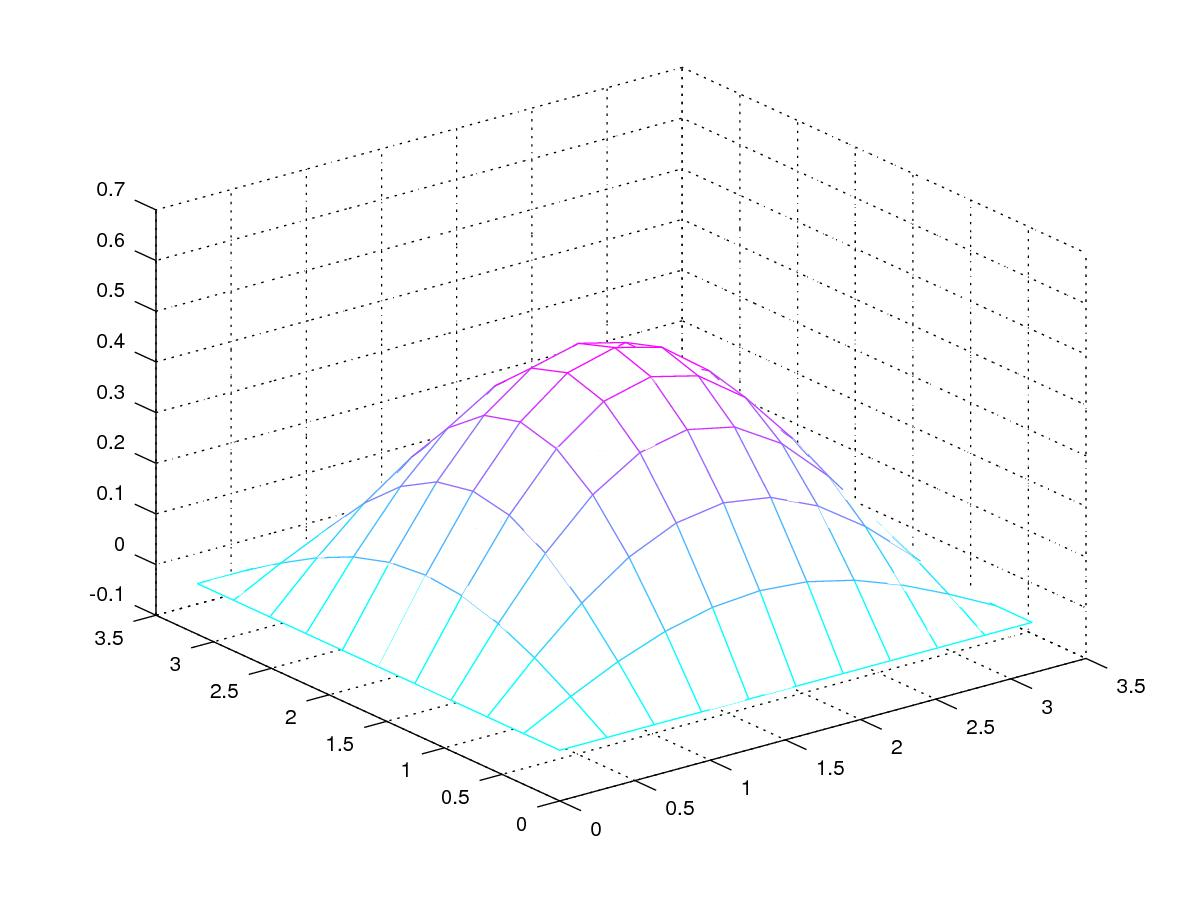
\includegraphics[width=0.8\textwidth]{./cap_edp/dados/ex_edp_Poisson/ex_edp_Poisson}
  \caption{Resultado referente ao Exemplo~\ref{ex:edp_Poisson}.}
  \label{fig:ex_edp_Poisson}
\end{figure}


A Figura~\ref{fig:ex_edp_Poisson} mostra um esboço do gráfico da solução aproximada obtida pelo método de diferenças finitas apresentado acima (equações \eqref{eq:edp_Poisson_mdf_sis0}-\eqref{eq:edp_Poisson_mdf_sis2}) com $n=11$, i.e. $h=\pi/10$.

\begin{table}[h!]
  \centering
  \begin{tabular}{l|c}
    $n$ & $\|\tilde{u}-u\|_{L^2}$\\\hline
    $6$ & $4,2\E-2$ \\
    $11$ & $2,1\E-2$ \\
    $21$ & $1,0\E-2$ \\
    $41$ & $5,1\E-3$ \\
    $81$ & $2,6\E-3$ \\\hline
  \end{tabular}
  \caption{Resultados referentes ao Exemplo~\ref{ex:edp_Poisson}.}
  \label{tab:ex_edp_Poisson}
\end{table}

Na Tabela~\ref{tab:ex_edp_Poisson} temos a norma $L^2$ da diferença entre a solução aproximada $\tilde{u}$ e a solução analítica $u(x,y) = 0,5\sen(x)\sen(y)$ nos pontos de malha computados com diferentes escolhas de $n$.

\ifisoctave
Os resultados obtidos neste exemplo podem ser obtidos no \verb+GNU Octave+ com o seguinte código:
\begin{verbatim}
#params
n=11;
h=pi/(n-1);

#fonte
f = @(x,y) -sin(x).*sin(y);

#malha
x = linspace(0,pi,n);
y = linspace(0,pi,n);

#sistema MDF
A = sparse(n*n,n*n);
b = zeros(n*n,1);

#cc x=0 e x=pi
for i=[1,n]
  for j=1:n
    k = i + (j-1)*n;
    A(k,k)=1;
    b(k) = 0;
  endfor
endfor

#cc y=0, y=pi
for j=[1,n]
  for i=1:n
    k = i + (j-1)*n;
    A(k,k)=1;
    b(k) = 0;
  endfor
endfor

#nodos internos
for i=2:n-1
  for j=2:n-1
    k = i + (j-1)*n;
    A(k,k-n) = 1/h^2;
    A(k,k-1) = 1/h^2;
    A(k,k) = -4/h^2;
    A(k,k+1) = 1/h^2;
    A(k,k+n) = 1/h^2;
    
    b(k) = f(x(i),y(j));
  endfor
endfor

u = A\b;

#visu
z = zeros(n,n);
for i=1:n
  for j=1:n
    k = i + (j-1)*n;
    z(i,j) = u(k);
  endfor
endfor
colormap("cool")
mesh(x,y,z)

ua = zeros(n*n,1);
for i=1:n
  for j=1:n
    k=i+(j-1)*n;
    ua(k) = 0.5*sin(x(i))*sin(y(j));
  endfor
endfor
printf("%d %1.5E %1.1E\n",n,h,norm(u-ua))
\end{verbatim}
\fi
\end{ex}

\subsection*{Exercícios}

\begin{exer}
  \begin{align}
    -(u_{xx} + u_{yy}) &= f(x),~(x, y)\in (0, 1)^2,\\
    u(0, y) &= 0,~y\in [0, 1],\\
    u(1, y) &= 0,~y\in [0, 1],\\
    \left.\frac{\p u}{\p y}\right|_{y=0} &= 0,~x\in [0, 1],\\
    u(x, 1) &= 0,~x\in [0, 1].
\end{align}
onde
\begin{equation}
  f(x) = \left\{
    \begin{array}{ll}
      1 &, x\leq 0,5\\
      0 &, x>0,5
    \end{array}
  \right.
\end{equation}
\end{exer}
Use uma aproximação adequada pelo método de diferenças finitas para obter o valor aproximado de $u(0,5,~0,5)$ com precisão de $2$ dígitos significativos.
\begin{resp}
  \ifisoctave 
  \href{https://github.com/phkonzen/notas/blob/master/src/MatematicaNumerica/cap_pvc/dados/exer_edp_Poisson_1/exer_edp_Possoin_1.m}{Código.} 
  \fi
  $2,9\E-2$
\end{resp}

\section{Equação do calor}\label{cap_edp_sec_calor}\index{equação!do calor}

A equação do calor definida em  $D = (x_{\text{ini}}, x_{\text{fin}})$ com condição inicial dada e condições de contorno de Dirichlet homogêneas refere-se o seguinte problema
\begin{align}
  u_t - \alpha u_{xx} &= f(t,x),~t>t_0,~x\in D, \label{eq:edp_calor_eq}\\
  u(t_0,x) &= u_0(x),~x\in D,\label{eq:edp_calor_ci}\\
  u(t, x_{\text{ini}}) &= 0,~t>t_0,\label{eq:edp_calor_bcxini}\\
  u(t, x_{\text{fin}}) &= 0,~t>t_0\label{eq:edp_calor_bcxfin}
\end{align}
onde $u = u(t,x)$ é a incógnita.

O problema acima é um problema de valor inicial com condições de contorno. Uma das estratégias numéricas de solução é o chamado método de Rothe, o qual trata separadamente as discretizações espacial e temporal. Aqui, vamos começar pela discretização espacial e, então, trataremos a discretização temporal.

\begin{flushleft}
  {\bf Discretização espacial}
\end{flushleft}

Na discretização espacial, aplicaremos o método de diferenças finitas. Começamos considerando uma partição do domínio $P(\overline{D}) = \{x_1, x_2, \dotsc, x_n\}$ com pontos $x_i = x_{\text{ini}}+(i-1)h$ igualmente espaçados por $h=(x_{\text{fin}}-x_{\text{ini}})$.  Então, denotando $u_{i}=u_{i}(t)\approx u(t,x_i)$ e usando da fórmula de diferenças finitas central de ordem $h^2$ para as derivadas segundas na equação \eqref{eq:edp_calor_eq}, temos
\begin{equation}
  \frac{\dd}{\dd t}u_{i} - \alpha\frac{u_{i-1}-2u_{i}+u_{i+1}}{h^2} = f(t,x_i),
\end{equation}
para $i=2, 3, \dotsc, n-1$. Agora, das condições de contorno, temos $u_1=0$ e $u_n=0$, donde obtemos o seguinte sistema de equações diferenciais ordinárias
\begin{align}\label{eq:edp_calor_disc_x1}
  \frac{\dd}{\dd t}u_2 &= -\frac{2\alpha}{h^2}u_{2} +\frac{\alpha}{h^2}u_{3} + f(t,x_2),\\
  \frac{\dd}{\dd t}u_i &= \frac{\alpha}{h^2}u_{i-1} - \frac{2\alpha}{h^2}u_{i} +\frac{\alpha}{h^2}u_{i+1} + f(t,x_i),\\
  \frac{\dd}{\dd t}u_{n-1} &= \frac{\alpha}{h^2}u_{n-2} - \frac{2\alpha}{h^2}u_{n-1}  + f(t,x_{n-1}),\\
\end{align}
onde $i=3, 4, \dotsc, n-2$ e com condições iniciais dadas por \eqref{eq:edp_calor_ci}, i.e.
\begin{equation}\label{eq:edp_calor_disc_x2}
  u_j(t_0) = u_0(x),~j=2, 3, \dotsc, n-1.
\end{equation}
Ainda, observamos que o sistema \eqref{eq:edp_calor_disc_x1} pode ser escrito de forma mais compacta como
\begin{equation}
  \frac{\dd \tilde{u}}{\dd t} = A\tilde{u} + \tilde{f},
\end{equation}
onde $\tilde{u}(t) = (u_2(t), u_3(t), \dotsc, u_{n-1}(t))$, $\tilde{f}(t) = (f(t,x_2), f(t,x_3), \dotsc, f(t,x_{n-1}))$ e $A$ é uma matriz $(n-2)\times (n-2)$ da forma
\begin{equation}\label{eq:edp_calor_disc_x3}
  A =
  \begin{bmatrix}
    -\frac{2\alpha}{h^2} & \frac{\alpha}{h^2} & 0 & 0 & 0 & \cdots & 0 & 0\\
    \frac{\alpha}{h^2} & -\frac{2\alpha}{h^2} & \frac{\alpha}{h^2} & 0 & 0 & \cdots & 0 & 0\\
    0 & \frac{\alpha}{h^2} & -\frac{2\alpha}{h^2} & \frac{\alpha}{h^2} & 0 & \cdots & 0 & 0\\
    0 & 0 & \ddots & \ddots & \ddots & \cdots & 0 & 0\\
    0 & 0 & & 0 & 0 & \cdots & \frac{\alpha}{h^2} & -\frac{2\alpha}{h^2}
  \end{bmatrix}.
\end{equation}


\begin{flushleft}
  {\bf Discretização temporal}
\end{flushleft}

Aqui, vamos usar o método de Euler (veja, \ref{cap_pvi_sec_Euler}) para aproximar a solução de \eqref{eq:edp_calor_disc_x3}-\eqref{eq:edp_calor_disc_x2}. Para tando, escolhemos um passo de tempo $h_t>0$ e denotamos $t^{(k)} = t_0 + (k-1)h_t$, $\tilde{u}^{(k)}\approx \tilde{u}(t^{(k)})$ e $\tilde{f}^{(k)} = \tilde{f}(t^{(k)})$. Com isso, a iteração do método de Euler nos fornece
\begin{align}
  \tilde{u}^{(1)} &= \tilde{u}_0\\
  \tilde{u}^{(k+1)} &= \tilde{u}^{(k)} + h_t\left(A\tilde{u}^{(k)}+\tilde{f}^{(k)}\right),
\end{align}
com $k=1, 2, \ldots$. Equivalentemente, escrevemos
\begin{align}
  \tilde{u}^{(1)} &= \tilde{u}_0\\
  \tilde{u}^{(k+1)} &= \left(I - h_tA\right)\tilde{u}^{(k)} + h_t\tilde{f}^{(k)}.
\end{align}

\begin{obs}
  O esquema numérico acima é \emph{condicionalmente estável}. Pode-se mostrar a seguinte condição de estabilidade \cite[Cap. 12, Seç. 2]{Burden2015a}:
  \begin{equation}
    \alpha\frac{h_t}{h^2}\leq \frac{1}{2}.
  \end{equation}
\end{obs}

\begin{ex}\label{ex:edp_calor}
  Consideremos o seguinte problema
  \begin{align}
    u_t - u_{xx} &= \sen(x),~t>0,~0\leq x \leq \pi,\\
    u(0,x) &= 0,~0<x<\pi,\\
    u(t,0) &= 0,~t>0\\
    u(t,\pi) &= 0,~t>0.
  \end{align}

\begin{figure}[h!]
  \centering
  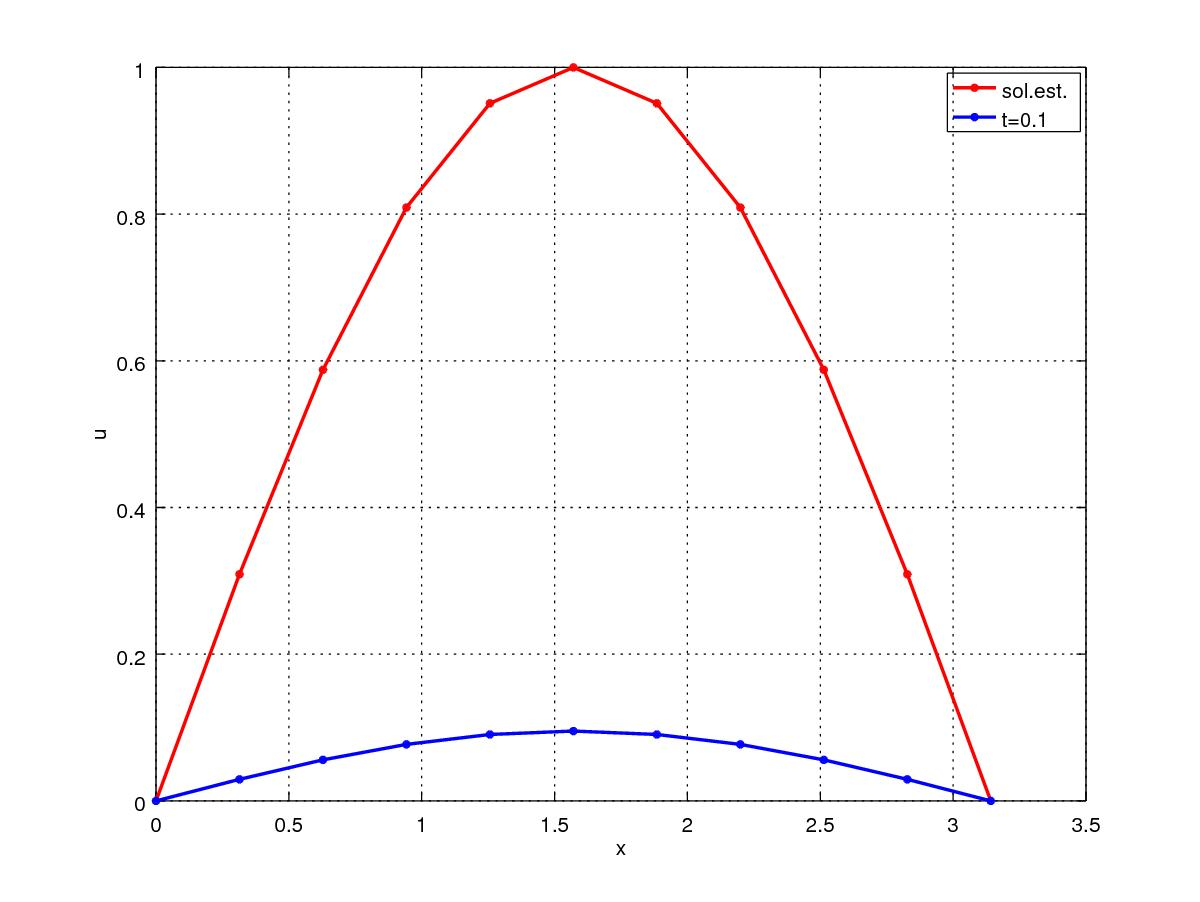
\includegraphics[width=0.45\textwidth]{./cap_edp/dados/ex_edp_calor/ex_edp_calor_t01} 
  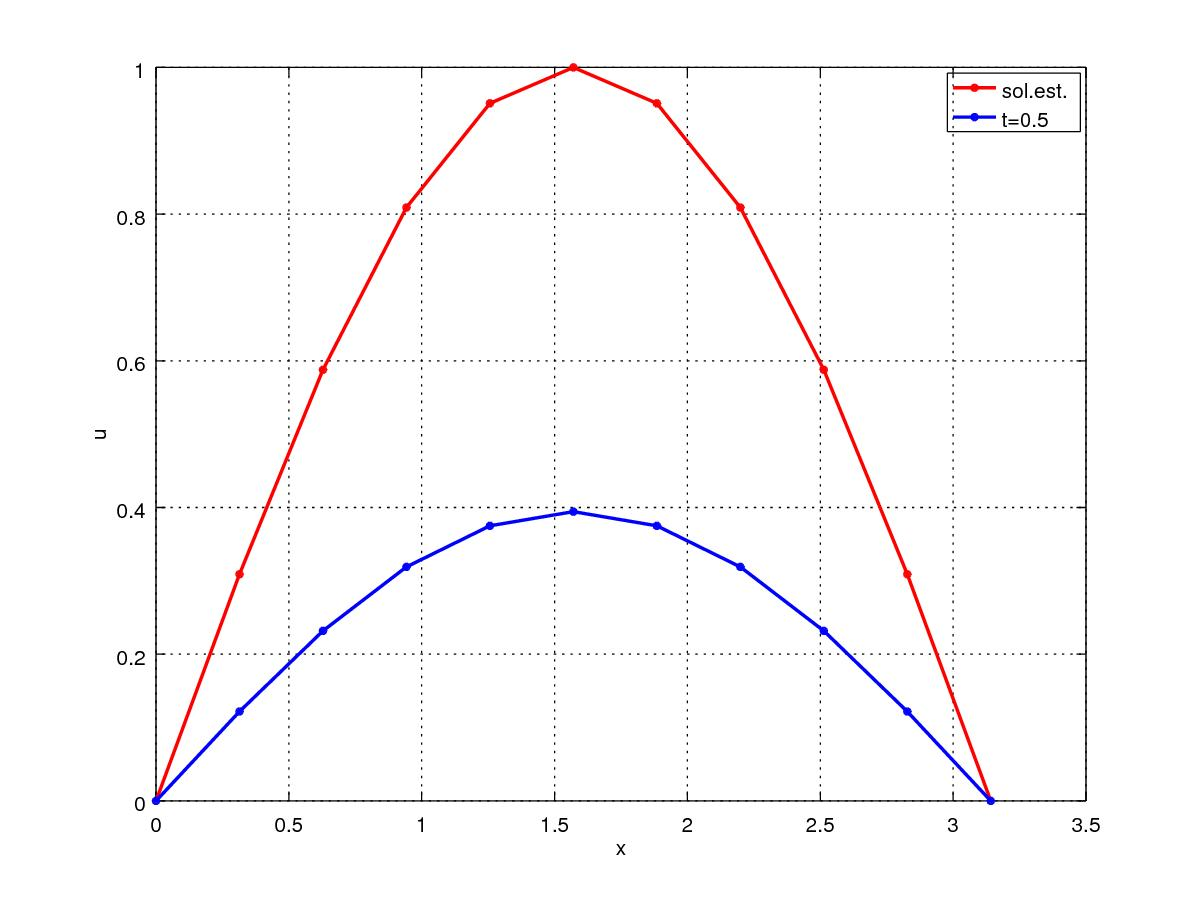
\includegraphics[width=0.45\textwidth]{./cap_edp/dados/ex_edp_calor/ex_edp_calor_t05}\\
  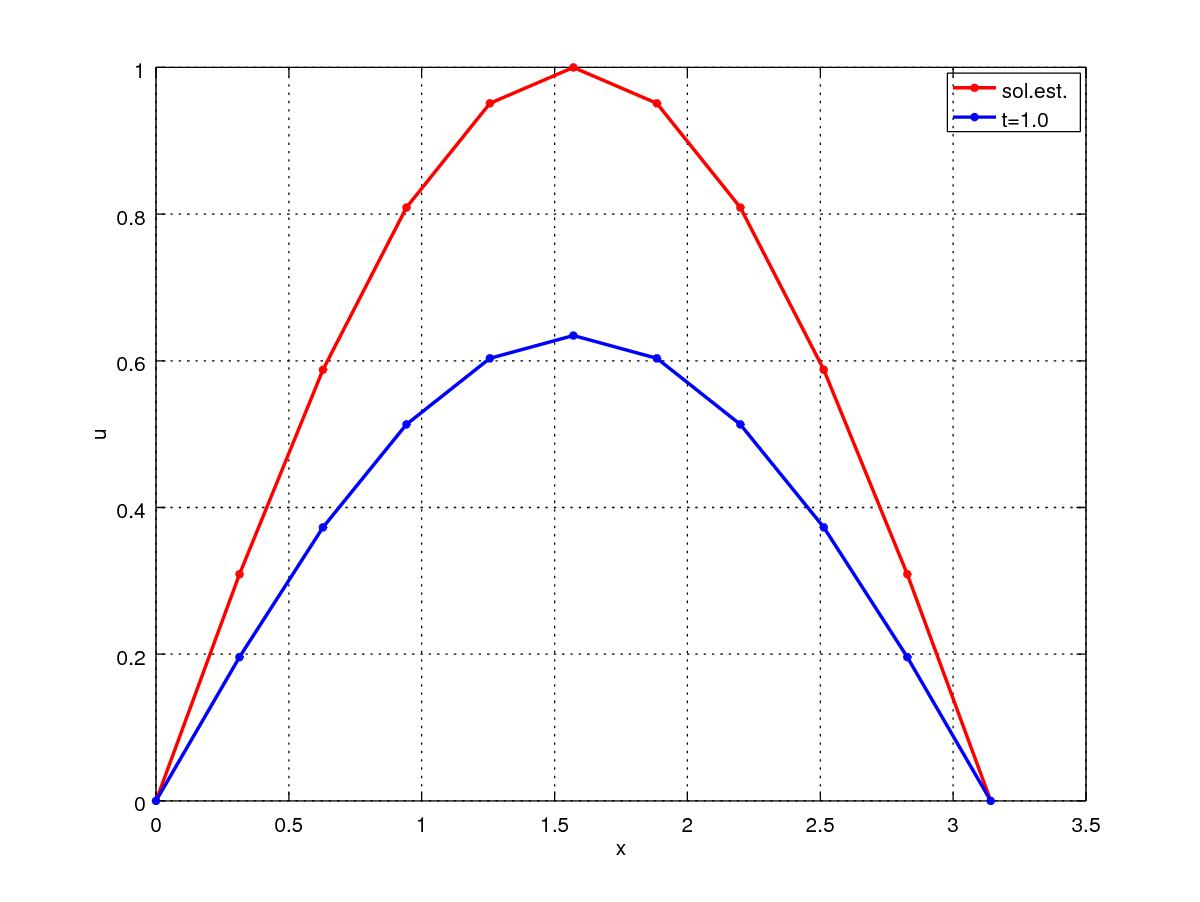
\includegraphics[width=0.45\textwidth]{./cap_edp/dados/ex_edp_calor/ex_edp_calor_t1} 
  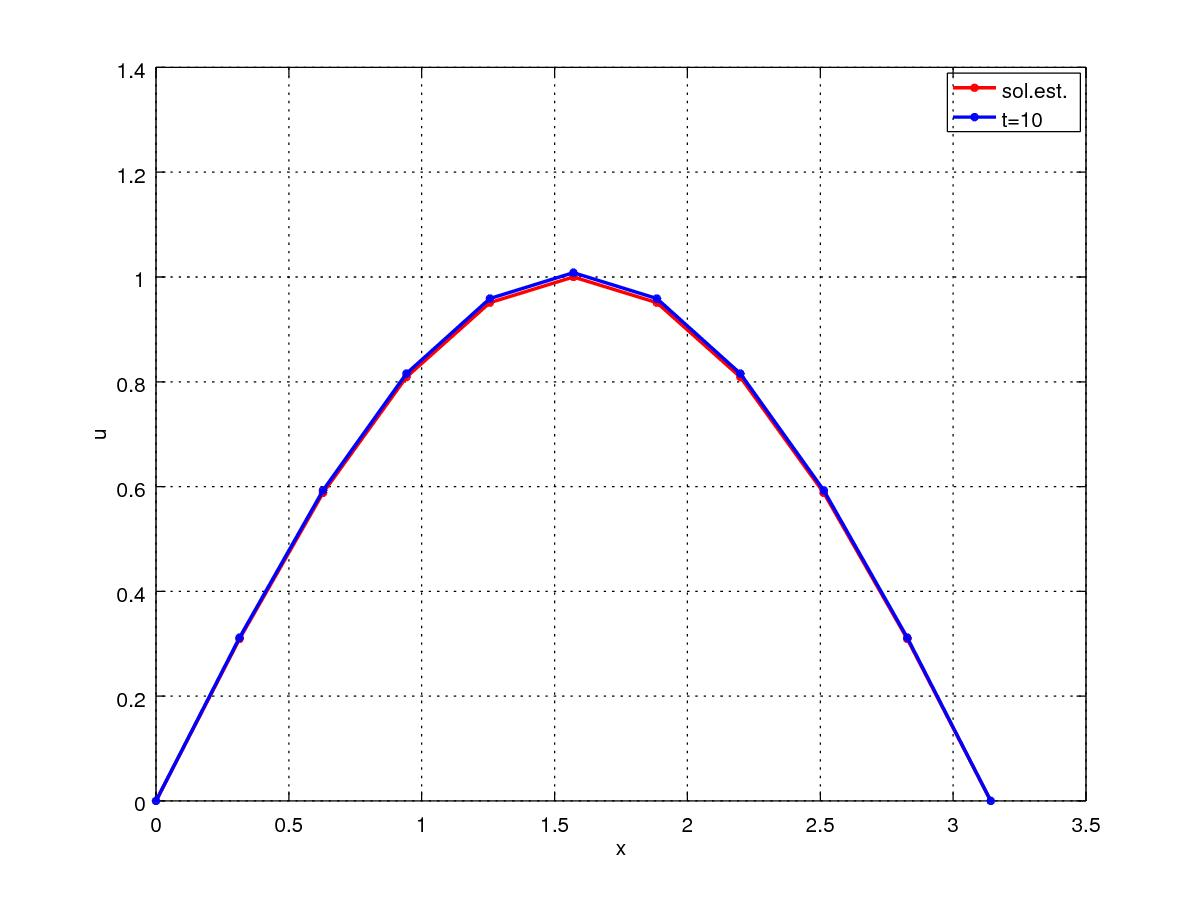
\includegraphics[width=0.45\textwidth]{./cap_edp/dados/ex_edp_calor/ex_edp_calor_t10}
  \caption{Resultados referentes ao Exemplo~\ref{ex:edp_calor}.}
  \label{fig:ex_edp_calor}
\end{figure}

Este problema tem solução estacionário $u(x) = \sen(x)$. Na Figura~\ref{fig:ex_edp_calor}, temos o esboço das soluções numéricas em diferentes tempos $t$ usando o esquema numérico acima com $h=10^{-1}$ e $h_t=10^{-3}$.

\ifisoctave
No \verb+GNU Octave+, podemos computar os resultados discutidos neste exemplo com o seguinte código:
\begin{verbatim}
#params
n=11;
h=pi/(n-1);

tf=1;
ht=10^-3;
nt=round(tf/ht)+1;

#fonte
f = @(x) sin(x);

#malha
t=[0:ht:(nt-1)*ht]'; 
x=[0:h:(n-1)*h]';

#matriz MDF
A = sparse(n-2,n-2);
A(1,1)=-2/h^2;
A(1,2)=1/h^2;
for i=2:n-3
  A(i,i-1)=1/h^2;
  A(i,i)=-2/h^2;
  A(i,i+1)=1/h^2;
endfor
A(n-2,n-3)=1/h^2;
A(n-2,n-2)=-2/h^2;

#c.i.
u=zeros(n,1);

#iter. de Euler
for k=1:nt-1
  u(2:n-1)=u(2:n-1)+ht*(A*u(2:n-1)+f(x(2:n-1)));
endfor

#visu
uest = @(x) sin(x);
plot(x,uest(x),'r.-',...
     x,u,'b.-');grid
xlabel('x');
ylabel('u');
legend('sol.est.','sol.num.');
\end{verbatim}
\fi
\end{ex}

\subsection*{Exercícios}

\begin{exer}
  Considere o seguinte problema
  \begin{align}
    u_t - u_{xx} &= f(x),~t>0,~0\leq x \leq 1,\\
    u(0,x) &= 0,~0<x<1,\\
    u(t,0) &= 1,~t>0\\
    u(t,1) &= 0,~t>0.
  \end{align}
com
\begin{equation}
  f(x) = \left\{
    \begin{array}{ll}
      1 &, x\leq 0,5,\\
      0 &, x>0,5
    \end{array}
\right.
\end{equation}
Use o método de diferenças finitas para obter uma aproximação de $u(1,0.5)$ com dois dígitos significativos de precisão.
\end{exer}
\begin{resp}
  \ifisoctave 
  \href{https://github.com/phkonzen/notas/blob/master/src/MatematicaNumerica/cap_edp/dados/exer_edp_calor_1/exer_edp_calor_1.m}{Código.} 
  \fi
  $5,6\E-1$
\end{resp}

\section{Equação da onda}\label{cap_edp_sec_onda}\index{equação!da onda}

A equação da onda definida em  $D := (x_{\text{ini}}, x_{\text{fin}})$ com condições iniciais dadas e condições de contorno de Dirichlet homogêneas refere-se o seguinte problema
\begin{align}
  u_{tt} - \alpha u_{xx} &= 0,~t>t_0,~x\in D, \label{eq:edp_onda_eq}\\
  u(x,t_0) &= f(x),~x\in D,\label{eq:edp_onda_ci1}\\
  \frac{\p u}{\p t}(x,t_0) &= g(x),~x\in D,\label{eq:edp_onda_ci2}\\
  u(x_{\text{ini}},t) &= 0,~t>t_0,\label{eq:edp_onda_bcxini}\\
  u(x_{\text{fin}},t) &= 0,~t>t_0\label{eq:edp_onda_bcxfin}
\end{align}
onde $u = u(x,t)$ é a incógnita.

Aqui, para aplicarmos o método de diferenças finitas, vamos escolher os tempos $t^{(j)} = t_0 + (j-1)h_t$, $j=1, 2, \dotsc, n_t$, com passo temporal $h_t>0$, e os pontos $x_i=x_{\text{ini}}+(i-1)h_x$, $i=1, 2, \dotsc, n_x$, com passo no espaço espacial $h_x = (x_{\text{fin}}-x_{\text{ini}})/(n_x-1)$.

Da escolha das discretizações temporal e espacial, podemos usar a fórmula de diferenças finitas de ordem $2$ para discretizarmos a equação \eqref{eq:edp_onda_eq}. Para tanto, denotamos $u_{i,j} \approx u(x_i,t_j)$ e de \eqref{eq:edp_onda_eq} temos
\begin{equation}
  \frac{u_{i,j-1}-2u_{i,j}+u_{i,j+1}}{h_t^2} - \alpha\frac{u_{i-1,j}-2u_{i,j}+u_{i+1,j}}{h_x^2} = 0,
\end{equation}
para $j=2, 3, \dotsc, n_t-1$ e $i=2, 3, \dotsc, n_x-1$. Rearranjando os termos, temos
\begin{equation}\label{eq:edp_onda_aux1}
  u_{i,j+1} = \alpha\frac{h_t^2}{h_x^2}u_{i-1,j} + 2\left(1-\alpha\frac{h_t^2}{h_x^2}\right)u_{i,j} + \alpha\frac{h_t^2}{h_x^2}u_{i+1,j} - u_{i,j-1},
\end{equation}
para $j=2, 3, \dotsc, n_t-1$ e $i=2, 3, \dotsc, n_x-1$.

Agora, das condições de contorno \eqref{eq:edp_onda_bcxini} e \eqref{eq:edp_onda_bcxfin}, temos $u_{1,j}=u_{n_x,j}=0$, $j=2, 3, \dotsc, n_t$. Com isso, o sistema \eqref{eq:edp_onda_aux1} torna-se
\begin{align}
  u_{2,j+1} &= 2\left(1-\alpha\frac{h_t^2}{h_x^2}\right)u_{2,j} + \alpha\frac{h_t^2}{h_x^2}u_{3,j} - u_{2,j-1},\\
  u_{i,j+1} &= \alpha\frac{h_t^2}{h_x^2}u_{i-1,j} + 2\left(1-\alpha\frac{h_t^2}{h_x^2}\right)u_{i,j} + \alpha\frac{h_t^2}{h_x^2}u_{i+1,j} - u_{i,j-1},\\
  u_{n_x-1,j+1} &= \alpha\frac{h_t^2}{h_x^2}u_{n_x-2,j} + 2\left(1-\alpha\frac{h_t^2}{h_x^2}\right)u_{n_x-1,j} - u_{i,j-1},\\
\end{align}
para $i=3, 4, \dotsc, n_x$ e $j=2, 3, \dotsc, n_t$. Este sistema de equações pode ser escrita na seguinte forma matricial
\begin{align}
  \begin{bmatrix}
    u_{2,j+1}\\
    u_{3,j+1}\\
    \vdots\\
    u_{n_x-1,j+1}
  \end{bmatrix}
  &=
  \begin{bmatrix}
    2(1-\lambda) & \lambda & 0 & \cdots & 0\\
    \lambda & 2(1-\lambda) & \lambda & \cdots & 0\\
    0  & \ddots & \ddots & \ddots & \cdots \\
    0  & 0 & \cdots & \lambda & 2(1-\lambda)
  \end{bmatrix}
  \begin{bmatrix}
    u_{2,j}\\
    u_{3,j}\\
    \vdots\\
    u_{n_x-1,j}
  \end{bmatrix}\nonumber\\
  &-
  \begin{bmatrix}
    u_{2,j-1}\\
    u_{3,j-1}\\
    \vdots\\
    u_{n_x-1,j-1}
  \end{bmatrix},\label{eq:edp_onda_iter3}
\end{align}
para $j=2, 3, \cdots, n_t-1$, onde $\lambda := \alpha h_t^2/h_x^2$.

Esta última equação~\eqref{eq:edp_onda_iter3} nos permite computar iterativamente a aproximação $u_{i,j+1}$ a partir das aproximações $u_{i,j}$ e $u_{i,j-1}$. Para inicializar as iterações, precisamos de $u_{i,1}$ e $u_{i,2}$, $i=2, 3, \dotsc, n_x$. A primeira é dada pela condição inicial \eqref{eq:edp_onda_ci1}, da qual temos
\begin{equation}\label{eq:edp_onda_iter1}
  u_{i,1} = f(x_i), ~i=2, 3, \dotsc, n_t.
\end{equation}
Agora, usando a fórmula de diferenças finitas progressiva de ordem $1$ na condições inicial \eqref{eq:edp_onda_ci2}, obtemos
\begin{equation}\label{eq:edp_onda_iter2}
  u_{i,2} = u_{i,1} + h_tg(x_i), ~i=2, 3, \dotsc, n_t.
\end{equation}

Com tudo isso, observamos que as equações \eqref{eq:edp_onda_iter1}, \eqref{eq:edp_onda_iter2} e \eqref{eq:edp_onda_iter3}, nesta ordem, nos fornece um algoritmo iterativo no tempo para computar as aproximações da solução $u$.

\begin{obs}
  Pode-se mostrar a seguinte condição de estabilidade
  \begin{equation}
    \alpha \frac{h_t^2}{h_x^2} \leq 1.
  \end{equation}
\end{obs}

\begin{ex}\label{ex:edp_onda}
  Consideremos o seguinte problema
  \begin{align}
    u_{tt} - u_{xx} &= 0,~t>0,~0< x < 1,\\
    u(0,x) &= x(1-x),~0<x<1,\\
    u_t(0,x) &= 0,~0<x<1,\\
    u(t,0) &= 0,~t>0\\
    u(t,\pi) &= 0,~t>0.
  \end{align}

\begin{figure}[h!]
  \centering
  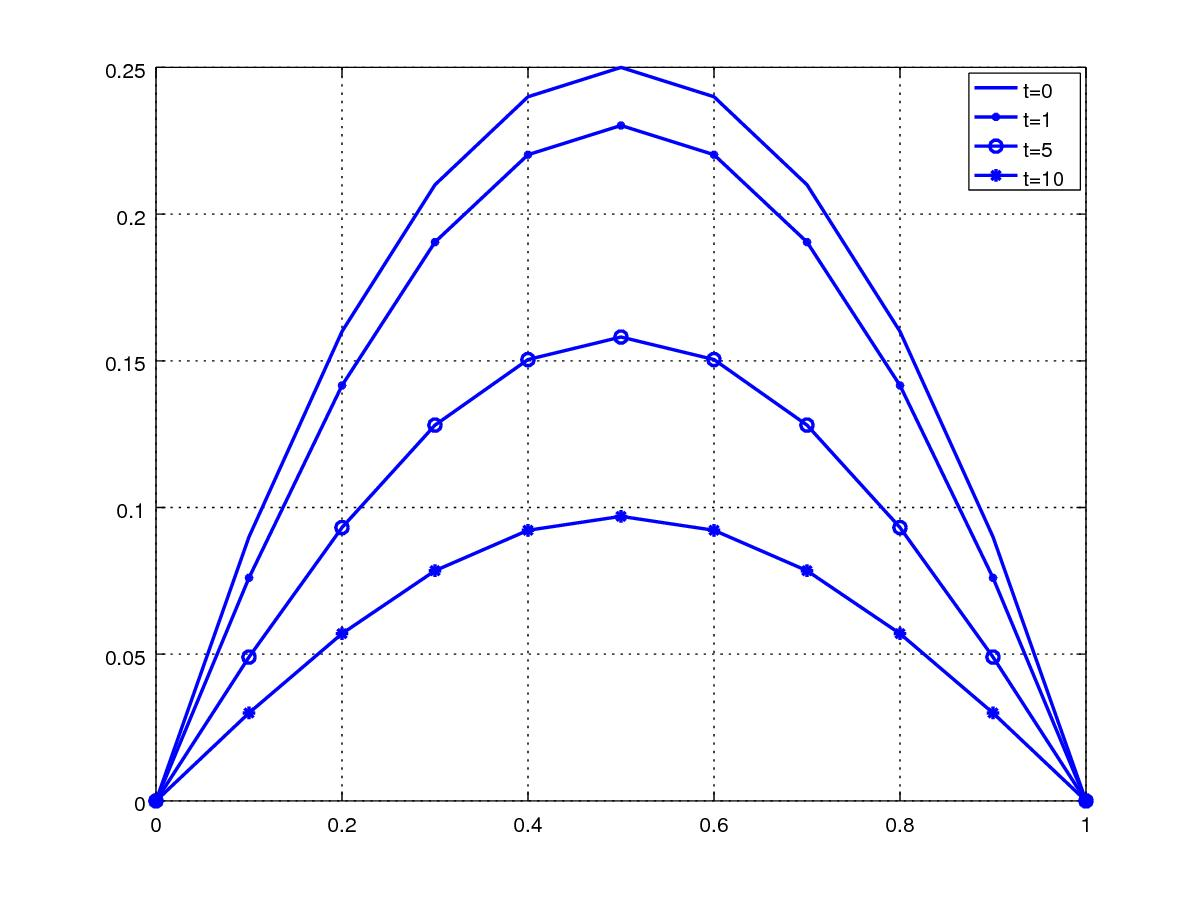
\includegraphics[width=0.8\textwidth]{./cap_edp/dados/ex_edp_onda/ex_edp_onda}
  \caption{Resultados referentes ao Exemplo~\ref{ex:edp_onda}.}
  \label{fig:ex_edp_onda}
\end{figure}

Na Figura~\ref{fig:ex_edp_onda}, temos o esboço das soluções numéricas em diferentes tempos $t$ usando o esquema numérico acima com $h_t=10^{-2}$ e $h_x=10^{-1}$.

\ifisoctave
No \verb+GNU Octave+, podemos computar os resultados discutidos neste exemplo com o seguinte código:
\begin{verbatim}
#params
nx=11;
hx=1/(nx-1);

tf=1;
ht=10^-2;
nt=round(tf/ht)+1;

lambda = ht^2/hx^2;

#malha
t=[0:ht:(nt-1)*ht]'; 
x=[0:hx:(nx-1)*hx]';

#u
u0=zeros(nx,1);
u1=zeros(nx,1);
u=zeros(nx,1);

#c.i. 1
for i=2:nx-1
  u0(i)=x(i)*(1-x(i));
endfor

#c.i. 2
u1=zeros(nx,1);
for i=2:nx-1
  u1(i)=u0(i)+ht*0;
endfor

#matriz MDF
A = sparse(nx-2,nx-2);
A(1,1)=2*(1-lambda);
A(1,2)=lambda;
for i=2:nx-3
  A(i,i-1)=lambda;
  A(i,i)=2*(1-lambda);
  A(i,i+1)=lambda;
endfor
A(nx-2,nx-3)=lambda;
A(nx-2,nx-2)=2*(1-lambda);

#iteracoes
for k=2:nt-1
  u(2:nx-1)=A*u1(2:nx-1) - u0(2:nx-1);
  u0=u1;
  u1=u;
endfor

#visu
plot(x,u1,'b-');grid
xlabel('x');
ylabel('u');
\end{verbatim}
\fi
\end{ex}

\subsection*{Exercício}

\begin{exer}
  Considere o seguinte problema
  \begin{align}
    u_{tt} - u_{xx} &= 0,~t>0,~0< x < 1,\\
    u(0,x) &= x(1-x),~0<x<1,\\
    u_t(0,x) &= 1,~0<x<1,\\
    u(t,0) &= 0,~t>0\\
    u(t,\pi) &= 0,~t>0.
  \end{align}
Use o método de diferenças finitas para obter uma aproximação de $u(0,75,~1)$ com dois dígitos significativos de precisão.
\end{exer}
\begin{resp}
  \ifisoctave 
  \href{https://github.com/phkonzen/notas/blob/master/src/MatematicaNumerica/cap_edp/dados/exer_edp_onda_1/exer_edp_onda_1.m}{Código.} 
  \fi
  $6,3\E-2$
\end{resp}